\documentclass{article}

% Language setting
% Replace `english' with e.g. `spanish' to change the document language
\usepackage[english]{babel}

% Set page size and margins
% Replace `letterpaper' with`a4paper' for UK/EU standard size
\usepackage[letterpaper,top=2cm,bottom=2cm,left=3cm,right=3cm,marginparwidth=1.75cm]{geometry}

% Useful packages
\usepackage{amsmath}
\usepackage{graphicx}
\usepackage[colorlinks=true, allcolors=blue]{hyperref}

\usepackage{algorithm}
\usepackage{algpseudocode}
\usepackage{amsmath}
\usepackage{amsfonts,amssymb}
\usepackage[shortlabels]{enumitem}
\usepackage{setspace}
\usepackage{tikz}




\title{CS229: Machine Learning}
\author{Junchuan Zhao}

\begin{document}
\setstretch{1.2} 
\maketitle

\begin{abstract}
This document includes my notes of CS229: Machine Learning.
\end{abstract}

\section{Lecture 2}
\subsection{Linear Regression}
Hypothesis: $h(x) = \sum\limits_{j=0}^n \theta_j x_j$ ($n$: number of features)

\noindent
Linear Regression: the hypothesis is the linear combination of the training dataset.

\noindent
Loss function (goal): $\min\limits_{\theta} \frac{1}{2} \sum\limits_{i=1}^m (h_{\theta}(x^i)-y^i)^2$

\noindent
Parameters: $\theta$, $m$, $n$, $x$, $y$

\subsection{Gradient Descent}
\subsubsection{Batch Gradient Descent}
Basic Ideas: start with some $\theta$, keep changing $\theta$ to reduce $J(\theta)$, repeat until convergent

\noindent
$\theta_j := \theta_j-\alpha\frac{\partial}{\partial \theta_j} J(\theta)$ ($\alpha$: learning rate)

\noindent
$\frac{\partial}{\partial \theta_j} J(\theta) = (h_\theta(x) - y) \cdot x_j$

\noindent
$\theta_j := \theta_j-\alpha \sum\limits_{i=1}^m (h_\theta(x)^i - y^i) \cdot x_j^i$ ($\alpha$: learning rate)

\noindent
Batch Gradient Descent: all the training data as a batch when optimizing the loss function.
(-): not good for large scale dataset, very expensive.

\subsubsection{Stochastic Gradient Descent}
\begin{algorithm}[h]
    \caption{Stochastic Gradient Descent}
  \label{alg::conjugateGradient}
  \begin{algorithmic}[1]
    \Require
    the parameter of $j^{th}$ feature
    \Ensure
    the updated parameter of $j^{th}$ feature
    \For {$i = 1$ to $m$}
        \State $\theta_j := \theta_j-\alpha \cdot (h_\theta(x)^i - y^i) \cdot x_j^i$;
    \EndFor
 
  \end{algorithmic}
\end{algorithm}

\noindent
stochastic gradient descent heads over to the global optimum.

\subsubsection{Total Equations}

A Total Equation for Stochastic Gradient Descent: $\nabla_{\theta}J(\theta) = \boldsymbol{0}$

\noindent
If A is square ($A \in \mathbb{R}_{n \times n}$)

Trace of A: $tr(A) = \sum\limits_{i}A_{ii}$

\noindent
Features of Trace:
\begin{itemize}[leftmargin=*, nosep]
    \item $tr(A) = tr(A^T)$
    \item $f(A) = tr(AB)$, $\nabla_{A}f(A) = B^T$
    \item $tr(AB) = tr(BA)$
    \item $tr(ABC) = tr(CAB)$
    \item $\nabla_{A}tr(AA^TC) = CA + C^TA$
\end{itemize}


~\\
\noindent
Loss Function: $\nabla_{\theta}J(\theta) = \frac{1}{2}(X\theta-y)^T(X\theta-y)$

\noindent
= $\frac{1}{2}(\theta^TX^T-y^T)(X\theta-y)$

\noindent
= $\frac{1}{2}(\theta^TX^TX\theta-\theta^TX^Ty-y^TX\theta)$

\noindent
= $X^TX\theta - X^Ty$

\noindent
Loss Function: $X^TX\theta - X^Ty = \boldsymbol{0}$ $\iff$ 
$X^TX\theta = X^Ty$

\noindent
$\theta = (X^TX)^{-1}X^Ty$

\section{Lecture 3}
\subsection{Locally Weighted Regression}
"Parametric" learning algorithm: fit fixed set of parameters ($\theta_i$) to data.

\noindent
"Non-parametric learning algorithm": amount of data/parameters you need to keep grows (linearly) with the size of data.

~\\
\noindent
Linear Regression: to evaluate $h$ at certain $x$

\noindent
Fit $\theta$ to minimize

$\frac{1}{2}\sum\limits_{i}(y^i-\theta^Tx^i)^2$, 

\noindent
return $\theta^Tx$


~\\
\noindent
Linear Regression: to evaluate $h$ at local region of $x$

\noindent
Fit $\theta$ to minimize

$\sum\limits_{i}w^i(y^i-\theta^Tx^i)^2$, 
where $w^i$ is a "weight function".

\noindent
common choice for $w^i$ is $w^i = e^{(-\frac{(x^i-x)^2}{2\tau^2})}$\\
If $\lvert x^i-x \rvert$ is small, then $w^i \approx 1$.\\
If $\lvert x^i-x \rvert$ is large, then $w^i \approx 0$.\\
$\tau$: bandwidth, control a larger or narrower window.\\

\subsection{Why Square Error?}

Assume $y^i = \theta^Tx^i + \epsilon^i$, where $\epsilon^i \sim  N(0, \sigma^2)$ models effects of random noise\\
$p(y^i|x^i;\theta) = \frac{1}{\sqrt{2\pi}\sigma}e^{-\frac{(y^i-\theta^Tx^i)^2}{2\sigma^2}}$\\
$\iff$ $y^i|x^i;\theta \sim N(\theta^Tx^i, \sigma^2)$\\

\noindent
Difference between Likelihood ($L$) and Probability ($P$): $L$ variess parameters, $P$ varies datapoints.
Assume the datapoints are IID,\\
The "likelihood" of $\theta$: $L(\theta) = p(\boldsymbol{y}|\boldsymbol{x};\theta)$
= $\prod\limits_{i=1}^m p(y^i|x^i;\theta)$\\
$l(\theta) = \log{\prod\limits_{i=1}^m\frac{1}{\sqrt{2\pi}\sigma}e^{(...)}}$
= $\sum\limits_{i=1}^m[\log{\frac{1}{\sqrt{2\pi}\sigma}} + \log{e^{(...)}}]$\\
= $m\log{\frac{1}{\sqrt{2\pi}\sigma}} - \sum\limits_{i=1}^m\frac{(y^i-\theta^Tx^i)^2}{2\sigma^2}$\\

\noindent
MLE: maximum likelihood estimation. Choose $\theta$ to maximize $L(\theta)$\\
i.e. choose $\theta$ to minimize $\frac{1}{2}\sum\limits_{i=1}^m(y^i-\theta^Tx^i)^2$, which is actually $J(\theta)$

\subsection{Classification}
Binary Classification: $y \in \{0,1\}$
\subsubsection{Logistic Regression}
We want $h_\theta(x) \in [0, 1]$, so we define\\
$h_\theta(x) = g(\theta^Tx) = \frac{1}{1 + e^{-\theta^Tx}}$\\
Sigmoid Function: $g(z) = \frac{1}{1 + e^{-z}}$\\
An important thing is that: the partial derivative of the sigmoid function is a \textbf{concave} function, which means it has the global maximum.
\begin{figure}[H]
	\centerline{
   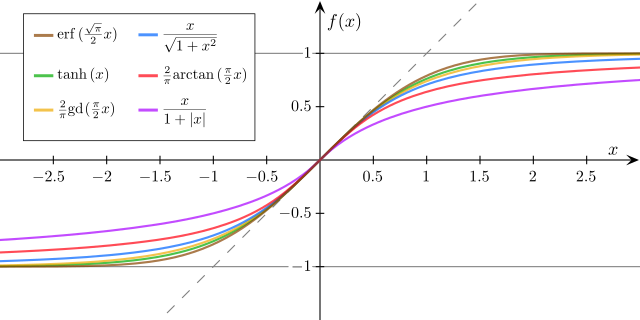
\includegraphics[width=0.5\textwidth]{Fig1.png}}
   \caption{The graph of sigmoid function.}
   \label{fig:example}
\end{figure}
\noindent
Different from Linear Regression $h_\theta(x) = \theta^Tx$, Logistic Regression is $h_\theta(x) = \frac{1}{1 + e^{-\theta^Tx}}$.\\
$p(y=1|x;\theta)=h_\theta(x)$, 
$p(y=0|x;\theta)=1-h_\theta(x)$\\
In sum, $p(y|x;\theta)=h_\theta(x)^y(1-h_\theta(x))^{1-y}$\\

\noindent
$L(\theta) = p(\boldsymbol{y}|\boldsymbol{x};\theta)$ = $\prod\limits_{i=1}^m h_\theta(x^i)^{y^i}(1-h_\theta(x^i))^{1-y^i}$\\
$l(\theta) = \log{(L(\theta))} = \sum\limits_{i=1}^m y^i\log{h_\theta(x^i)} + (1-y^i)\log{(1-h_\theta(x^i))}$\\
Choose $\theta$ to maximize $l(\theta)$, we use Batch gradient ascent.\\

\noindent
Batch Gradient Ascent:\\
\indent
$\theta_j := \theta_j + \alpha\frac{\partial}{\partial\theta_j}l(\theta)$\\
$\theta_j := \theta_j + \alpha\sum\limits_{i=1}^m(y^i-h_\theta(x^i))x_j^i$, same as the one in linear regression. (A larger category called generalized linear model (GLM))\\
Note: no \textbf{normal equation} for logistic regression solution.\\

\subsubsection{Newton's Method}
The basic idea: have some function $f$, we want to fit $\theta$, \textbf{s.t.} $f(\theta)=0$ $\iff$ want maximizing $l(\theta)$ $\iff$ want $l'(\theta)=0$\\
\begin{figure}[H]
	\centerline{
   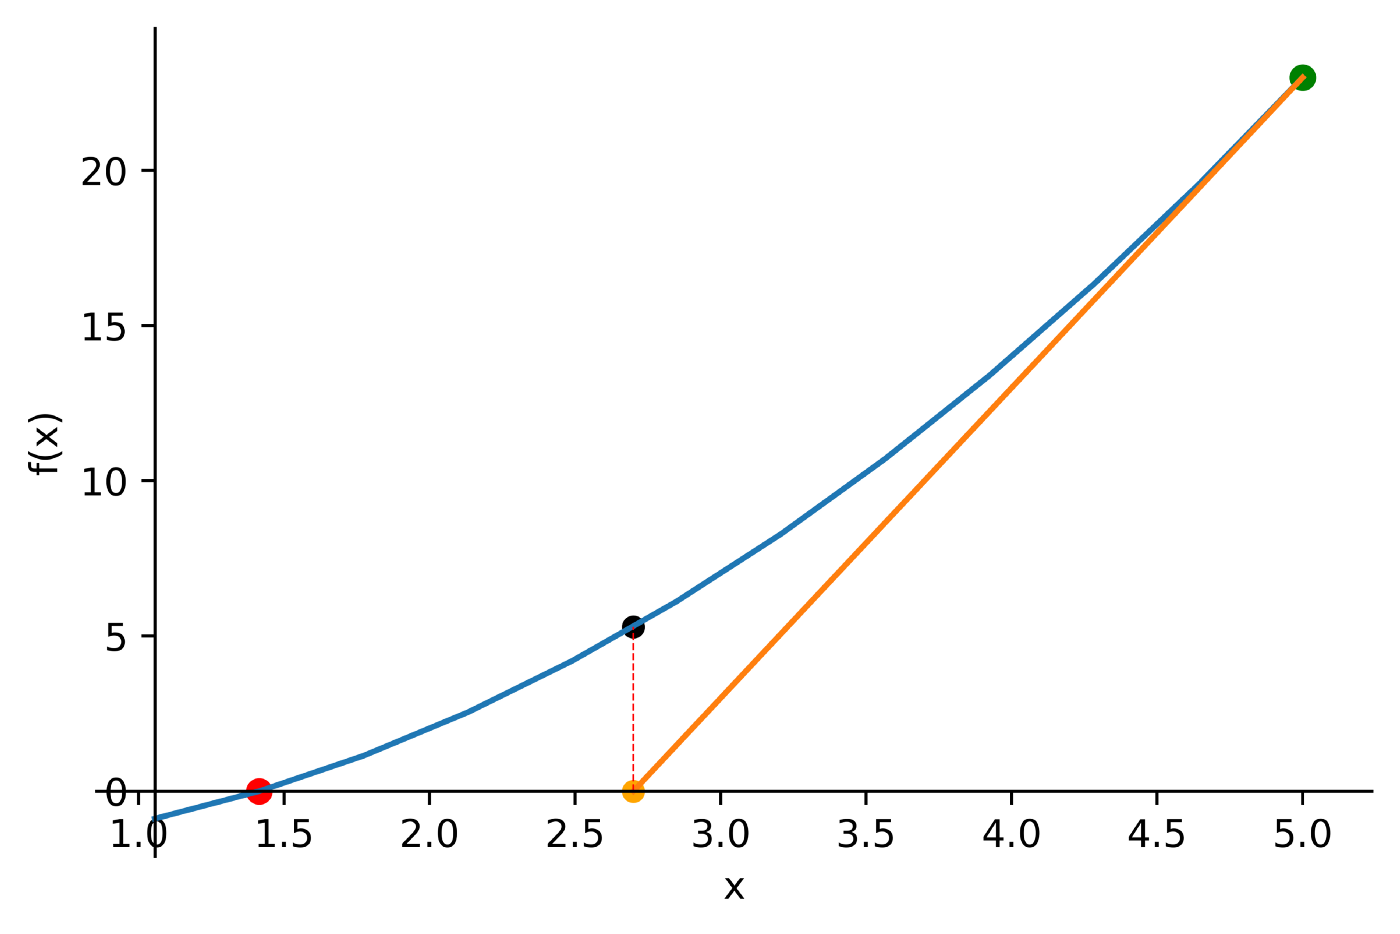
\includegraphics[width=0.5\textwidth]{Fig2.png}}
   \caption{Newton's Method.}
   \label{fig:example}
\end{figure}
\noindent
$\theta^{t+1} := \theta^{t} - \frac{f(\theta^t)}{f^{'}(\theta^t)}$, let $f(\theta) = l^{'}(\theta)$\\
$\theta^{t+1} := \theta^{t} - \frac{l^{'}(\theta^t)}{l^{''}(\theta^t)}$\\

\noindent
"\textbf{Quadratic convergent}": $0.01$ error $\longrightarrow$ $0.0001$ error $\longrightarrow$ $0.00000001$ error.\\

\noindent
When $\theta$ is a vector: ($\theta \in \mathbb{R}^{n+1}$)\\
\indent
$\theta^{t+1} := \theta^t + \alpha H^{-1}\nabla_\theta l(\theta)$\\
where 
$$
\nabla_\theta l(\theta) = 
\begin{bmatrix}
  \frac{\partial l}{\partial\theta_{00}} & \frac{\partial l}{\partial\theta_{01}} & \cdots & \frac{\partial l}{\partial\theta_{0n}} \\
  \frac{\partial l}{\partial\theta_{10}} & \frac{\partial l}{\partial\theta_{11}} & \cdots & \frac{\partial l}{\partial\theta_{1n}} \\
  \vdots & \vdots  & \ddots & \vdots \\
  \frac{\partial l}{\partial\theta_{n0}} & \frac{\partial l}{\partial\theta_{n1}} & \cdots & \frac{\partial l}{\partial\theta_{nn}} \\
\end{bmatrix}
$$
$H \in \mathbb{R}^{n+1 \times n+1}$ is the Hessian Matrix, $H_{ij} = \frac{\partial^2l}{\partial\theta_i\partial\theta_j}$\\
Note: If the dataset is large, the size of $H$ will be too large to compute.
\indent


\end{document}